\documentclass[a4paper,14pt]{extarticle} \usepackage[utf8]{inputenc}
\usepackage[T1]{fontenc}
\usepackage[margin=2.5cm]{geometry}

% Fonte Caladea se existir, senão lmodern
\IfFileExists{caladea.sty}{
  \usepackage{caladea}
}{
  \usepackage{lmodern} }
\usepackage{ragged2e}
\usepackage{graphicx}
\usepackage[portuguese]{babel}
\usepackage{wrapfig}
\usepackage{hyperref}
\usepackage{fancyhdr}
\usepackage{xcolor}
\usepackage{rotating}
\usepackage{titlesec}
\usepackage{epigraph}
\usepackage{dirtytalk}
\usepackage{indentfirst} % Indenta o primeiro parágrafo após seções

% Ajuste do recuo de parágrafo
\setlength{\parindent}{1.5em}

% Centralizar títulos
\titleformat{\section}
  {\normalfont\centering\bfseries\Large}{\thesection}{1em}{}

\titleformat{\subsection}
  {\normalfont\centering\bfseries\large}{\thesubsection}{1em}{}

\titleformat{\subsubsection}
  {\normalfont\centering\bfseries}{\thesubsubsection}{1em}{}

% -------------- Símbolos de Versículo e Resposta --------------
% Definição do símbolo (a “barrinha” inclinada)
\makeatletter
\newcommand{\vers@resp@sym}{%
  \raisebox{0.2ex}{\rotatebox[origin=c]{-20}{$\m@th\rceil$}}%
}
% macro interna que sobrepõe a barrinha e a letra V ou R
\newcommand{\vers@resp}[2]{%
  {\ooalign{%
     \hidewidth\kern#1\vers@resp@sym\hidewidth\cr
     #2\cr
  }}%
}
% comandos públicos \versicle e \response
\DeclareRobustCommand{\versicle}{\vers@resp{-0.1em}{V}}
\DeclareRobustCommand{\response}{\vers@resp{0pt}{R}}
\makeatother
% ^------------- Símbolos de Versículo e Resposta -------------^

% Rodapé com imagem e página
\pagestyle{fancy}
% ---- Cabeçalho ------------
\fancyhf[C]{}
% ----- Rodapé --------------
\fancyfoot[LO,LE]{%
  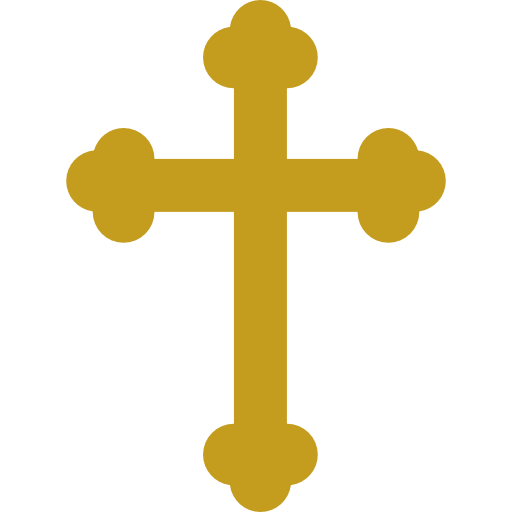
\includegraphics[scale=0.2]{assets/cross.png}\quad
  \textit{Novena a \textbf{São Martinho de Lima}}
}
\fancyfoot[RO,RE]{\thepage}

\begin{document}


\begin{center}
  {\huge Novena a São Martinho de Lima}
\end{center}

\say{
Existem depoimentos de pessoas que o viram entrar e sair de lugares cujas portas estavam trancadas e testemunhos que asseguram tê-lo visto em dois lugares diferentes ao mesmo tempo: é o fenômeno da bilocação.
}

\par\noindent\rule{\textwidth}{0.4pt}

\tableofcontents
\thispagestyle{empty}

% --- Vida / Origem da Novena ---
\newpage

\section{História}

Hoje a Igreja faz memória de São Martinho de Lima, um contemporâneo de outra exímia alma esposa de Deus, Santa Rosa de Lima.

Martinho nasceu em Lima, Peru, no dia 9 de dezembro de 1579, e foi batizado na Igreja de San Sebastián, mesmo local do batismo de Rosa de Lima. Seus pais chamavam-se Ana Velasquez, uma panamenha de origem africana, e Juan de Porres, um nobre espanhol. Ele foi beatificado em 1837 por Gregório XVI. Segundo o Papa João XXIII, Martinho foi “uma resposta da Igreja para os problemas e questões raciais do século XX.”

\subsection{Os movimentos da graça e o despertar vocacional}

Seu chamado à vida religiosa aconteceu em sua juventude. Procurou então o prior do Convento de Nossa Senhora do Rosário, pedindo que o aceitasse como frade. Na época, as normas canônicas e as da própria Ordem dos Dominicanos não admitiam o ingresso de recém convertidos, nativos e mestiços, nem descendentes até a quarta geração. Negros e mulatos tambem estavam nas mesmas condições excludentes.

Entretanto, Martinho gozava de uma ótima reputação e estima entre os frades daquele convento, por isso, o prior solicitou ao Provincial autorização para que o “mulato” fosse admitido como um “irmão donato”, ou seja, sem votos públicos. Desse modo, São Martinho dedicou-se aos cuidados domésticos do convento. Por causa desse ofício, em algumas obras artísticas é representado com uma vassoura nas mãos. Quando foi encarregado de trabalhar no na enfermaria do convento, tornou-se símbolo de amparo aos pobres e doentes. Com o passar do tempo, sua humildade e bondade valeram-lhe o respeito e a estima de toda a cidade, até que seu ingresso oficial na ordem foi concedido. Seus superiores, entusiasmados, disputavam o privilégio de presidir o rito de sua profissão solene como religioso.

\subsection{Grande virtude da humildade}

Apesar de se julgar indigno, Martinho fez sua profissão religiosa no dia 2 de junho de 1603, consagrando-se a Deus. Ele nunca se despojou das vestes que recebeu nesse dia. Usava os mesmos hábitos, já velhos, assim como seus sapatos gastos. Seu único luxo era o de trazer dois rosários, um no pescoço e outro preso ao cinto de couro. A única vez que Martinho aceitou um hábito novo, gesto que deixou todos surpresos, foi quando expressou que a sua morte estava próxima, o que de fato ocorreu no dia 3 de novembro de 1639.

Os milagres ocorridos por suas mãos começaram a acompanhá-lo já em vida, tanto que o superior lhe proibiu de fazê-los, pois grande era a movimentação das pessoas no convento, o que perturbava a paz do lugar. É famoso um episódio em que estava caminhando pela rua e viu um homem cair de um andaime. Vendo o ocorrido, gritou para que o homem parasse no ar e correu para o mosteiro para pedir autorização ao seu superior para fazer o milagre de salvar a vida do homem. Seu superior assentiu e ele voltou para fazê-lo cair suavemente ao chão, sem nenhum ferimento. Vários milagres também atribuídos aos méritos de Martinho diante de Deus foram constatados já nos primeiros instantes após sua páscoa. Como quando seu corpo perdeu a rigidez própria de um cadáver e várias e várias pessoas receberam a cura e a libertação de seus males.

\subsection{O reconhecimento público da Igreja}

A causa da beatificação de Martinho foi introduzida em 1664, mas somente em 1837 foi declarado beato. O processo de canonização foi reaberto em 1926. Aprovado no terceiro e último consistório, o beato foi finalmente declarado santo pela Igreja, sendo aprovados seu ofício litúrgico e orações próprias nas devoções e missas em sua memória. 

Que Deus abençoe toda a Igreja da América Latina por intercessão de São Martinho. Que seu testemunho e intercessão contribuam para o crescimento da fé em todo o continente americano. 

São Martinho, rogai por nós!  

% --- Orações Diárias ---
\newpage

\section{Novena a São Martinho de Lima}

\subsection{Oração Inicial} \label{oracao-inicial}

Ó São Martinho de Lima, escutai hoje nossos pedidos, nossas tristezas e arrependimentos, seja nosso consolo. Nos nossos obstáculos e adversidades, ajudai- nos. Em nossas maiores tentações, cubra-nos. Com doença e o arrependimento, ajudai-nos.
Oh, bondoso Santo, imploramos por uma solução para nossas necessidades, tira qualquer mal de nós, afasta de nós o mentiroso, protege nossa casa e nossa família, ouça nosso pedido, São Martinho.
(Fazer o pedido).
Poderoso São Martinho de Porres, pelos milagres que realizou na vida, pela misericórdia que demonstrou, pela humildade que transbordou e pela glória que desfruta ao lado do Senhor, conceda-nos este pedido.
Compassivo São Martinho, sei que entende nossos problemas, sei que nos ajudará, confiamos em vós. Milagroso São Martinho, cubra nossos passos e não nos deixe cair
em tentações, acompanhe-nos em nossos sucessos e ajudai-nos em nossos lamentos. Amém.

\subsection{Oração Final} \label{oracao-final}

Rezar Pai-Nosso, Ave-Maria e Glória ao Pai.

\[
\textbf{São Martinho de Lima, rogai por nós!}
\]

\vfill

\begin{center}
\subsection*{Fontes:}
Adaptado de: \underline{\href{https://comshalom.org/sao-martinho-de-lima-o-santo-que-venceu-todas-as-barreiras-pela-via-do-amor/}{Comunide Shalom}} e \underline{\href{https://www.scribd.com/document/742970466/Novena-a-Sao-Martinho-de-Porres}{Novena a São Martinho dos Porres}}.
\end{center}


\end{document}
